
\documentclass[a4paper]{article}
\usepackage{authblk}
\usepackage{array}
\usepackage{amsmath}
\usepackage{amssymb}
\usepackage{amsfonts}
\usepackage{amscd}
\usepackage{tikz}
\usetikzlibrary{snakes,arrows,shapes}
\usepackage{graphicx}
\usepackage{caption}
\usepackage{appendix}
\usepackage{hyperref}
\usepackage[utf8]{inputenc}
\usepackage[round]{natbib}
\usepackage{bm}
%\usepackage{chemist}
%\usepackage{chemformula}
\usepackage{breqn}
\usepackage{enumitem}
\usepackage{setspace} %needed for preprint in doublelinespace 
%\usepackage[colorinlistoftodos, textwidth=4cm, shadow]{todonotes} %comments and
\usepackage[normalem]{ulem} % provides strike out
%\usepackage[draft,multiuser]{fixme} %change draft to final for the final version
%\FXRegisterAuthor{cs}{acs}{CS} 
%creating special annotation commands \csnote \cswarning .. and environments \acsfor Carlos
%\FXRegisterAuthor{mm}{amm}{MM} 
%\usepackage[round]{natbib}
\newtheorem{definition}{Definition}
\DeclareRobustCommand{\Rbb}[1]{
		\mathbb{R}^{+^{#1}}
}
\DeclareRobustCommand{\ubar}[1]{\text{\b{$#1$}}}

\DeclareRobustCommand{\diag3}[3]{
	\left(
		\begin{matrix}
		#1	& 0  		& \cdots	 & 0 \\
		0 	& \ddots	& \ddots 	 & \vdots \\
		\vdots 	& \ddots 	& \ddots 	 & 0 \\
		0 	& \cdots        & 0		 & #3\\
		\end{matrix}
	\right) 
}
\DeclareRobustCommand{\triang2}[2]{
	\left(
		\begin{matrix}
		#1_{1,1}#2	& 0 		& \cdots	 & 0 \\
		\vdots	 	& \ddots	& \ddots 	 & \vdots \\
		\vdots 		& 	 	& \ddots 	 & 0 \\
		#1_{n,1}#2	& \cdots        & \cdots	 & #1_{n,n}#2\\
		\end{matrix}
	\right) 
}
\DeclareRobustCommand{\Fbb}[1]{
		\mathcal{F}
		\left(
			\mathbb{T},\mathbb{R}^{+^{#1}}
		\right) 
}
\DeclareRobustCommand{\Rbb}[1]{
		\mathbb{R}^{+^{#1}}
}

\DeclareRobustCommand{\RN}[1]{
	\textup{\uppercase\expandafter{\romannumeral#1}}%
}

\DeclareRobustCommand{\Mathbox}[2]{
	\text{
		\parbox[t][#1][t]{6cm}{
			\small{#2}
		}
	}
}
%\DeclareRobustCommand{\vec}[1]{\mathbf{#1}}
%\DeclareRobustCommand{\mat}[1]{\mathbf{#1}}
\DeclareRobustCommand{\figref}[1]{ Fig. \ref{#1}}
\DeclareRobustCommand{\revref}[1]{Comment: \ref{#1}}
\DeclareRobustCommand{\Theoref}[1]{Theorem \ref{#1}}
\DeclareRobustCommand{\Defref}[1]{\mbox{Definition \ref{#1}}}
\DeclareRobustCommand{\enumref}[1]{\ref{#1}}
\DeclareRobustCommand{\appendixref}[1]{appendix \ref{#1}}
\DeclareRobustCommand{\Appendixref}[1]{Appendix \ref{#1}}
\DeclareRobustCommand{\sectionref}[1]{ section \ref{#1}}
\DeclareRobustCommand{\tupelref}[2]{\enumref{#1} \enumref{#2}}
%\definecolor{dark-green}{rgb}{0,0.25,0}
\hypersetup{
    colorlinks=true,
    linkcolor=blue,
    filecolor=magenta,      
    urlcolor=blue,
    %pdftitle={Sharelatex Example},
    bookmarks=true,
    %pdfpagemode=FullScreen,
}

\title{The python packages CompartmentalSystems, LAPM  and bgc-md}
\date{\today}
\author[1]{Ver{\'{o}}nika Ceballos-N{\'{u}}{\~{n}}ez}
\author[1]{Holger Metzler}
\author[1]{M{arkus M{\"{u}}ller}}
\author[1]{Carlos A. Sierra}
\affil[1]{Max Planck for Biogeochemistry, Hans-Knöll-Str. 10, 07745 Jena, Germany}

\begin{document}
\maketitle

\section{People and Contributions}
\newenvironment{mmpage}{
\begin{minipage}[t]{\textwidth}
	\begin{flushleft}
}
{
	\end{flushleft}
\end{minipage}
\vspace{0.2mm}
}
The presented Software is the fruit of genuine teamwork. 
To be able to compete in the categories of group leaders, postdocs and Ph.D. students 
we give a simplified summary.

\begin{table}[ht]
	\begin{tabular}{l|p{2.5cm}|p{4cm}}
		\bf{Name}
		& 
		\begin{mmpage}
		\bf{Position}
		\end{mmpage}
		& 
		\begin{mmpage}
		\bf{Contributions}
		\end{mmpage}
		\\
		\hline
		Ver{\'{o}}nika Ceballos-N{\'{u}}{\~{n}}ez 	
		& 
		\begin{mmpage}
		Ph.D. student 
		\end{mmpage}
		& 
		\begin{mmpage}
		database population \\
		report generation \\
		abstract vegetation model 
		\end{mmpage}
		\\
		\hline
		Holger Metzler					
		& 
		\begin{mmpage}
		Ph.D. student 
		\end{mmpage}
		&
		\begin{mmpage}
		algorithm development, \\
		implementation, testing, \\
		database population \\
		report generation 
		\end{mmpage}
		\\
		\hline
		Markus Müller 					
		& 
		\begin{mmpage}
		postdoc, \\
		developer 
		\end{mmpage}
		& 
		\begin{mmpage}
		technical lead, \\
		algorithm development, \\
		implementation, testing, \\
		report generation, \\
		refactoring, infrastructure 
		\end{mmpage}
		\\
		\hline
		Carlos Sierra					
		& 
		\begin{mmpage}
		postdoc,\\
		 group-leader 
		\end{mmpage}
		&
		\begin{mmpage}
		abstract models, \\
		database population, \\
		outside collaboration, \\
		organization, funding 
		\end{mmpage}
	\end{tabular}
\end{table}

\section{Introduction}
The presented software framework consists of three open source python packages, 
that serve to represent, classify and analyse compartmental systems of ordinary differential equations (see \Defref{def:compartmentalModel} in \Appendixref{App:Models})with special emphasis on the computation of age and transit time densities of the content.  
The packages do not have a graphical user interface and are meant to be used together with other open source software e.g. \href{jupyter.org}{jupyter}. 

\subsection{CompartmentalSystems package}
\url{https://github.com/MPIBGC-TEE/CompartmentalSystems}\\
The package allows the computation of ages and transit times for nonlinear, non autonomous well mixed compartmental systems.
A brief summary if found under the link above. A more detailed description of the concepts and their application is given in \citet[]{MetzlerMuellerSierra2018PNAS}. A preprint is attached \url{./PNAS.pdf}.
An example \href{jupyter.org}{jupyter} notebook that shows how to use the package can be found here:
\url{http://compartmentalsystems.readthedocs.io/en/latest/_downloads/nonl_gcm_3p.html}

\subsection{LAPM package}
\url{https://github.com/MPIBGC-TEE/LAPM}\\

\subsection{The biogeochemical model data base}
\url{https://github.com/MPIBGC-TEE/bgc-md}\\
Short summaries are found under the link above or on our group website \url{https://www.bgc-jena.mpg.de/TEE/software/bgc-md/}.
The package provides: 
\begin{enumerate} 
	\item
	Collections of \href{https://github.com/MPIBGC-TEE/bgc-md/tree/master/bgc_md/data/all_records}{yaml files} each encoding a published carbon cycling model  
	
	\item 
		The code to produce (at the moment still static) \href{https://www.bgc-jena.mpg.de/TEE/software/bgc-md/vegetation/list_report_v.html}{html} for user specified queries or can be used in a \href{https://github.com/MPIBGC-TEE/bgc-md/blob/master/jupyter_notebooks/Examples/how_to_apply_toolkit_to_yaml_model.ipynb}{jupyter notebook}. 
\end{enumerate} 
The software simplifies the abstract description of element cycling models and introduces a yaml format to store them. It uses a symbolic mathematical representation based on \href{http://www.sympy.org/en/index.htmlhttp://www.sympy.org/en/index.html}{sympy} but also allows immediate numerical computations using numpy and our own packages. 
Its main use is to make complex models immediately available for further investigation e.g. in jupyter notebooks, but it also provides a command-line tool to build html reports about single models or sets. Users can create their own templates.
Although we are developing a web front end that makes it possible to run the whole database as a website with a graphical JavaScript based user interface, so that further simplifies the creation of the database entries the main use case right now is to create a yaml file describing a model  an produce static html reports.




\begin{appendices}
\section{Compartmental systems}
\label{App:Models}
For the purpose of understanding the applications of the software it suffices to interpret
all state variables as contents of reservoirs.
In the following we treat here reservoir, pool, and compartmental systems as synonymous, 
and use relevant definitions from \citet[][and references therein]{Jacquez1993SIAM}. 
The interpretation easiest to imagine is content measured in units of mass stored in a reservoir defined by its spatial boundaries.
However, reservoirs as well as contents can be much more abstract. 
\begin{definition}[Compartmental system]
	\label{def:compartmentalModel} 
	Let 
	$F_{i,j}$  be the flux from pool $j$  to pool $i ,\text{ for all } i,j\ne i \in \{1 \dots n \}$,
	$F_{i,0}=I_i$ define the influx to pool $i$ 
	and 
	$F_{0,i}=O_i$ the outflux from pool $i$. \\ 
	If 
	$F_{i,j}(\vec{C},t)	\ge  0 ,\text{ for all } i,j \in \{0 \dots n\} $ and
	\begin{align}
	\label{enum:ZeroFlux}	
	C_j=0 			\implies  F_{i,j}(\vec{C},t)=0
	\end{align}
	we call the ODE system: 
	\begin{align}
	\label{eq:internalMassBalance}
	\dot{C}_i=	\sum_{i=0.i\ne j}(-F_{j,i}(\vec{C},t)+F_{i,j}(\vec{C},t)) \quad{\forall i}
	\end{align}
	\emph{compartmental}.
\end{definition}
\begin{figure}[h]
        %\def\svgwidth{\columnwidth}
	%\input{3PoolsFeedBackWaterM.pdf_tex}
	%\includegraphics[width=.5\textwidth]{3PoolsFeedBackWaterM.pdf}

	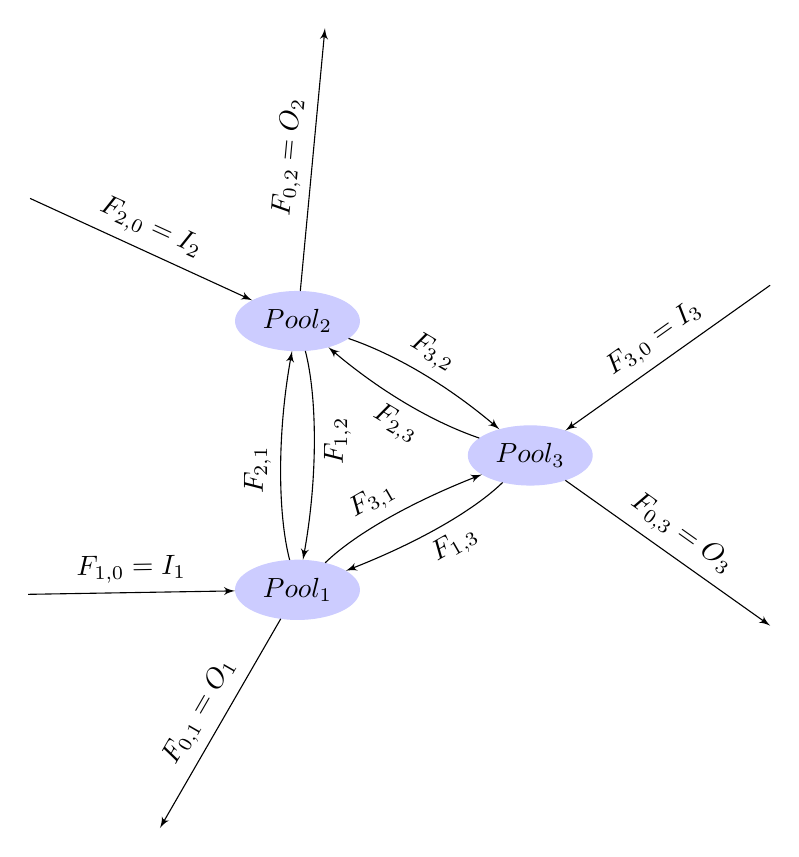
\begin{tikzpicture}[>=latex',line join=bevel,]
	%%
	\node (p2) at (279.93bp,200.49bp) [draw=blue!20,fill=blue!20,ellipse] {$Pool_2$};
	  \node (p3) at (363.73bp,152.12bp) [draw=blue!20,fill=blue!20,ellipse] {$Pool_3$};
	  \node (p1) at (279.93bp,103.74bp) [draw=blue!20,fill=blue!20,ellipse] {$Pool_1$};
	  \coordinate (o3) at (450.09bp,90.839bp);
	  \coordinate (o1) at (230.43bp,18.0bp);
	  %\coordinate (e1) at (27.0bp,152.12bp);
	  \coordinate (e1) at (183.0bp,102.12bp);
	  \coordinate (o2) at (289.82bp,305.92bp);
	  \coordinate (e3) at (450.09bp,213.39bp);
	  \coordinate (e2) at (183.68bp,244.65bp);
	
	  \definecolor{strokecol}{rgb}{0.0,0.0,0.0};
	  \pgfsetstrokecolor{strokecol}
	  \draw [->] (e3) -- node[above,sloped]{$F_{3,0}=I_3$}(p3);
	  \draw [->] (p3) -- node[above,sloped]{$F_{0,3}=O_3$}(o3);
	
	  \draw [->] (e2) -- node[above,sloped]{$F_{2,0}=I_2$}(p2);
	  \draw [->] (p2) -- node[above,sloped]{$F_{0,2}=O_2$}(o2);
	
	  \draw [->] (e1) -- node[above,sloped]{$F_{1,0}=I_1$}(p1);
	  \draw [->] (p1) -- node[above,sloped]{$F_{0,1}=O_1$}(o1);
	
	  \draw [->] (p1) ..controls (299.33bp,122.68bp) 	and (318.25bp,134.21bp)	.. node[above,sloped]{$F_{3,1}$}(p3);
	  \draw [->] (p3) ..controls (344.33bp,133.17bp) 	and (325.41bp,121.64bp)	.. node[below,sloped]{$F_{1,3}$}(p1);
	
	  \draw [->] (p2) ..controls (286.97bp,173.65bp) 	and (287.36bp,144.53bp)	.. node[below,sloped]{$F_{1,2}$}(p1);
	  \draw [->] (p1) ..controls (272.89bp,130.58bp) 	and (272.5bp,159.7bp)  	.. node[above,sloped]{$F_{2,1}$}(p2);
	  
	  \draw [->] (p2) ..controls (314.37bp,188.75bp) 	and (333.26bp,177.94bp) .. node[above,sloped]{$F_{3,2}$} (p3);
	  \draw [->] (p3) ..controls (329.29bp,163.86bp) 	and (310.4bp,174.67bp) 	.. node[below,sloped]{$F_{2,3}$}(p2);
	%
	\end{tikzpicture}
	\caption{
     	\label{fig:3PoolsFeedBackWaterM}
	A compartmental model with three pools and all possible
	connections between the pools and the environment.  
	%The fluxes between pools
	%$F_{k,l}(\vec{C}$,$t) \ge 0 $ with  $F_{k,l}(\vec{C}$,$t) =0$ for
	%$C_k=0 $ 
	%are a necessary part of the definition.  
	Note that the flux between pool$_k$ and pool$_l$ is considered a property of the
	\emph{pipeline}, meaning the flux from pool$_k$ into the pipeline is the
	same as the flux out of the pipeline into pool$_k$.  
	This ensures mass balance for all fluxes and pools and also for the model as a whole, and
	makes this the prototype or normal form of mass balanced models with
	internal connections.  
	Every model that can be drawn in this
	form is mass balanced.  Examples are not limited to networks of
	pipelines and reservoirs of fluids. Instead of a fluid the total amount
	of a chemical element in different chemical substances (represented by
	the pools) can be described by it.
	}
\end{figure}
Remarks:\\
The conditions guarantee mass balance, non-negative fluxes,
and ensure that there cannot be any flux out of an empty pool.
For non-negative initial values $\vec{C}_0\in \Rbb{n}$ the pool contents stay non-negative for  $t\ge t_0$.
\end{appendices}

\bibliography{/home/mm/SoilR/Bibliography/TEE}
\bibliographystyle{apa}
%\bibliography{../../../Bibliography/TEE}
\begin{enumerate}
		\item
			usage examples for bgc-md that work
		\item 
			automated tests that make sure that all the models in data/
		\item 
\end{enumerate}
\end{document}
